\documentclass[preview]{standalone}

\usepackage{amsmath}
\usepackage{amssymb}
\usepackage{stellar}
\usepackage{definitions}
\usepackage{bettelini}
\usepackage{tikz}
\usetikzlibrary{patterns,arrows.meta}

\begin{document}

\id{divergence-theorem-applications}
\genpage

\section{Divergence Theorem Applications}

\begin{snippetexample}{coulomb-field-flux-example}{Flux of a Coulomb field}
    Let
    \[
        E(x,y,z)=\nabla\left(
        -\frac{kq}{\sqrt{x^2+y^2+z^2}}
        \right),
    \]
    and let \(\Omega\subseteq\realnumbers^3\) be a bounded admissible
    domain containing the origin. Compute the outward flux of \(E\) through
    \(\partial\Omega\).
\end{snippetexample}

\begin{snippetsolution}{coulomb-field-flux-solution}{Flux of a Coulomb field}
    The divergence theorem cannot be applied directly to \(\Omega\), since
    \(E\) is singular at the origin. Choose \(R>0\) such that
    \(\overline{B_R(0)}\subseteq\Omega\), and set
    \(D=\Omega\setminus\overline{B_R(0)}\). If
    \[
        u(x,y,z)=-\frac{kq}{\sqrt{x^2+y^2+z^2}},
    \]
    then \(E=\nabla u\) and \(\Delta u=0\) away from the origin. Thus
    \[
        0=\iiint_D\operatorname{div}E
        =\int_{\partial\Omega}E\cdot\nu_e\,dS
        -\int_{\partial B_R(0)}E\cdot\nu_e\,dS.
    \]
    The minus sign occurs because the normal of the inner boundary points
    into the removed ball. On \(\partial B_R(0)\),
    \[
        E=\frac{kq}{R^3}(x,y,z),
        \qquad
        \nu_e=\frac{(x,y,z)}R,
    \]
    so \(E\cdot\nu_e=kq/R^2\). Consequently,
    \[
        \int_{\partial\Omega}E\cdot\nu_e\,dS
        =\frac{kq}{R^2}\,4\pi R^2
        =4\pi kq.
    \]
\end{snippetsolution}

\begin{snippetexample}{outward-flux-solid-example}{Outward flux from a solid}
    Compute the outward flux of
    \[
        F(x,y,z)=
        ye^{x+y}\mathbf i-xe^{x+y}\mathbf j+xy\mathbf k
    \]
    through the boundary of
    \[
        \Omega=
        \{(x,y,z):|y|\leq x\leq2-|y|,\ 0\leq z\leq x+y\}.
    \]
\end{snippetexample}

\begin{snippetsolution}{outward-flux-solid-solution}{Outward flux from a solid}
    Since
    \[
        \operatorname{div}F=(y-x)e^{x+y},
    \]
    the divergence theorem gives
    \[
        \int_{\partial\Omega}F\cdot\nu_e\,dS
        =\iint_T(x+y)(y-x)e^{x+y}\,dx\,dy,
    \]
    where
    \[
        T=\{(x,y):|y|\leq x\leq2-|y|\}.
    \]

    \begin{center}
        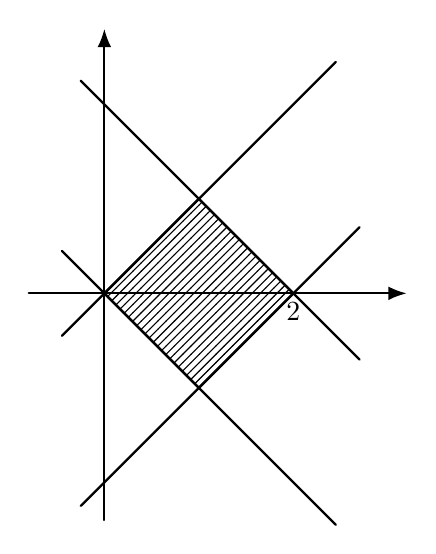
\begin{tikzpicture}[scale=1.2,>=Latex,line cap=round,line join=round]
            \draw[->,thick] (-0.8,0) -- (3.2,0);
            \draw[->,thick] (0,-2.4) -- (0,2.8);

            \fill[pattern=north east lines,pattern color=black]
            (0,0) -- (1,1) -- (2,0) -- (1,-1) -- cycle;

            \draw[thick] (0,0) -- (1,1) -- (2,0) -- (1,-1) -- cycle;

            \draw[thick] (-0.25,2.25) -- (2.7,-0.7);
            \draw[thick] (-0.25,-2.25) -- (2.7,0.7);

            \draw[thick] (-0.45,-0.45) -- (2.45,2.45);
            \draw[thick] (-0.45,0.45) -- (2.45,-2.45);

            \node[below] at (2,0) {\(2\)};
        \end{tikzpicture}
    \end{center}

    Introduce
    \[
        u=x+y,
        \qquad v=x-y.
    \]
    Then \(0\leq u,v\leq2\),
    \(dx\,dy=\tfrac12du\,dv\), and
    \((x+y)(y-x)e^{x+y}=-uve^u\). Therefore
    \begin{align*}
        \int_{\partial\Omega}F\cdot\nu_e\,dS
        &=-\frac12
        \left(\integral[0][2][ue^u][u]\right)
        \left(\integral[0][2][v][v]\right)\\
        &=-\frac12(e^2+1)\cdot2\\
        &=-(e^2+1).
    \end{align*}
\end{snippetsolution}

\end{document}
